\documentclass{article}
\usepackage[margin=1in]{geometry}  % Helps with proper margins
\usepackage{amsmath}               % For mathematical symbols and align environment
\usepackage{graphicx}              % For including images
\usepackage{amssymb}               % For additional symbols

\begin{document}

\section*{A9}

\subsection*{(c)}

The runtime differences between the vanilla and numpy implementations for varying sizes of \(n\) are summarized below:

\[
\begin{array}{|c|c|c|}
\hline
n & \text{Vanilla Implementation (ms)} & \text{Numpy Implementation (ms)} \\
\hline
20   & 0.999   & 0.0 \\
200  & 18.978  & 1.9981 \\
500  & 177.8502 & 0.0 \\
1000 & 531.933 & 1.0056 \\
\hline
\end{array}
\]

\paragraph{Explanation:}
The vanilla implementation is significantly slower compared to the numpy implementation because it relies on Python loops for matrix multiplication and vector operations, which are less efficient. Numpy, on the other hand, uses highly optimized C and Fortran libraries for linear algebra computations, which execute operations in a much faster and parallelized manner.

\begin{figure}
    \centering
    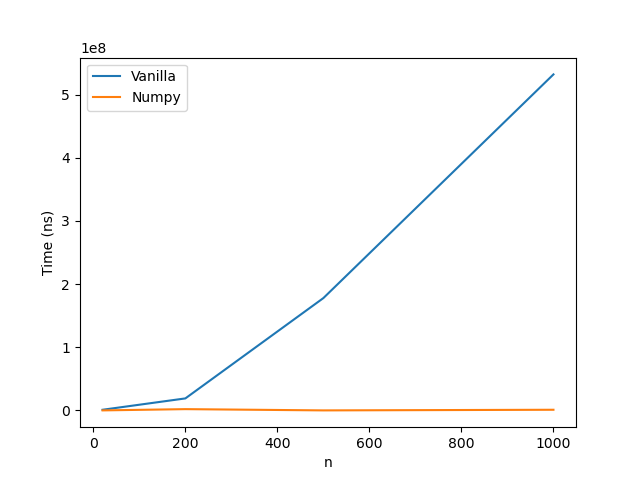
\includegraphics[width=0.5\linewidth]{C:/Users/admin/Downloads/ML/hw0/hw0-tex/van_vs_numpy_figure.png}
    \caption{Runtime comparison of vanilla vs. numpy implementations for varying sizes of \(n\).}
    \label{fig:van-vs-numpy}
\end{figure}

\end{document}